\begin{figure}[tb]
\centering
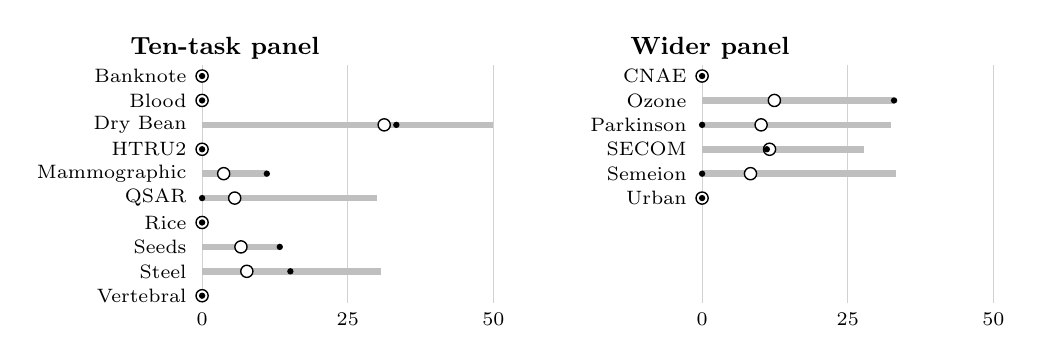
\begin{tikzpicture}[x=.074cm,y=.31cm,font=\scriptsize]
\foreach \offset/\heading in {0/{Ten-task panel},6.35/{Wider panel}}{
\begin{scope}[xshift=\offset cm]
\node[anchor=west,font=\small\bfseries] at (-14,11.15) {\heading};
\foreach \x in {0,25,50}{
 \draw[gray!35,thin] (\x,0.7)--(\x,10.45);
 \node[anchor=north] at (\x,.7) {\x};
}
\end{scope}}
\foreach \y/\name/\point/\lottery/\ceiling in
 {10/Banknote/0/0/0,9/Blood/0/0/0,8/{Dry Bean}/33.333/31.250/50,
  7/HTRU2/0/0/0,6/Mammographic/11.111/3.704/11.111,5/QSAR/0/5.598/29.966,
  4/Rice/0/0/0,3/Seeds/13.333/6.667/13.333,2/Steel/15.152/7.677/30.707,1/Vertebral/0/0/0}{
 \node[anchor=east] at (-1,\y) {\name};
 \draw[line width=2.4pt,gray!50] (0,\y)--(\ceiling,\y);
 \draw[black,fill=white,line width=.5pt] (\lottery,\y) circle[radius=2.2pt];
 \fill[black] (\point,\y) circle[radius=1.15pt];}
\begin{scope}[xshift=6.35cm]
\foreach \y/\name/\point/\lottery/\ceiling in
 {10/CNAE/0/0/0,9/Ozone/32.946/12.403/32.946,8/Parkinson/0/10.127/32.340,
  7/SECOM/11.111/11.574/27.778,6/Semeion/0/8.305/33.221,5/Urban/0/0/0}{
 \node[anchor=east] at (-1,\y) {\name};
 \draw[line width=2.4pt,gray!50] (0,\y)--(\ceiling,\y);
 \draw[black,fill=white,line width=.5pt] (\lottery,\y) circle[radius=2.2pt];
 \fill[black] (\point,\y) circle[radius=1.15pt];}
\end{scope}
\end{tikzpicture}
\caption{Fraction of anchor columns saved within tolerance (percent), averaged over each task's folds. A gray bar ends at the largest attainable mean with the prescribed guard. Open circles mark the exact expected return under uniform nomination and solid dots the point margin. A dot inside a circle indicates matching values. On Parkinson and Semeion some candidate could pass both checks, yet point recovered none of those opportunities.}
\label{fig:opportunity}
\end{figure}
